% Use the following line _only_ if you're still using LaTeX 2.09.
%\documentstyle[icml2015,epsf,natbib]{article}
% If you rely on Latex2e packages, like most modern people use this:
\documentclass{article}

% use Times
\usepackage{times}
% For figures
\usepackage{graphicx} % more modern
\graphicspath{ {images/} }
\usepackage{subfigure} 

% For citations
\usepackage{natbib}

% For algorithms
\usepackage{algorithm}
\usepackage{algorithmic}

% As of 2011, we use the hyperref package to produce hyperlinks in the
% resulting PDF.  If this breaks your system, please comment out the
% following usepackage line and replace \usepackage{icml2015} with
% \usepackage[nohyperref]{icml2015} above.
\usepackage{hyperref}

% Packages hyperref and algorithmic misbehave sometimes.  We can fix
% this with the following command.
\newcommand{\theHalgorithm}{\arabic{algorithm}}

% Employ the following version of the ``usepackage'' statement for
% submitting the draft version of the paper for review.  This will set
% the note in the first column to ``Under review.  Do not distribute.''
\usepackage{icml2015} 

% Employ this version of the ``usepackage'' statement after the paper has
% been accepted, when creating the final version.  This will set the
% note in the first column to ``Proceedings of the...''
%\usepackage[accepted]{icml2015}


% The \icmltitle you define below is probably too long as a header.
% Therefore, a short form for the running title is supplied here:
\icmltitlerunning{Recurrent Generative Stochastic Networks for Sequence Prediction}

\begin{document} 

\twocolumn[
\icmltitle{Recurrent Generative Stochastic Networks for Sequence Prediction}

% It is OKAY to include author information, even for blind
% submissions: the style file will automatically remove it for you
% unless you've provided the [accepted] option to the icml2015
% package.
\icmlauthor{Markus Beissinger}{markusb@wharton.upenn.edu}
\icmladdress{University of Pennsylvania, 220 South 33rd Street, Philadelphia, PA 19104 USA}
\icmlauthor{Lyle Ungar}{ungar@cis.upenn.edu}
\icmladdress{University of Pennsylvania, 220 South 33rd Street, Philadelphia, PA 19104 USA}

% You may provide any keywords that you 
% find helpful for describing your paper; these are used to populate 
% the "keywords" metadata in the PDF but will not be shown in the document
\icmlkeywords{deep learning, sequence, RNN, GSN, generative}

\vskip 0.3in
]


\begin{abstract} 
	This is the abstract.
\end{abstract} 


\section{Introduction}
\label{introduction}
Unsupervised sequence learning is an important problem in machine learning given that most information (ranging from speech to video to even consumer behavior) is often unlabeled and has a sequential structure. Most of these sequences consist of high-dimensional, complex objects such as words in text, images in video, or chords in music. Recently, recurrent neural networks (RNN) \cite{rnn} have become state-of-the-art for sequence representation because they have an internal memory that can learn long-term, temporal dependencies. Further advances with Hessian-free optimization and Long Short-term Memory for RNNs \cite{hessian_free, lstm} have enabled learning highly complex temporal dependencies.

While traditional RNNs can learn complex sequences through maintaining an internal memory, they don't deal well when modeling complex input distributions, where the conditional distribution at each time step is highly multi-modal. In real-world data, we often care more about this conditional distribution rather than the expected value. In music, for example, the existence of a particular note can highly change the probabilities with which other notes occur at the same time in a chord. In consumer behavior, the existence of a particular action taken can highly change the probabilities of other actions made within the same time window. We would prefer to reason over these distributions at each time step to form a better representation of the sequences.

Deep RNN architectures have been proposed to alleviate the traditional architecture shortcomings with complex input distributions \cite{deep_rnn}. One proposed framework involves using deep input-to-hidden and hidden-to-output functions to reduce input complexity, making the RNN's task easier.

\cite{rnnrbm}

In Sections 2, 3, and 4, we introduce the GSN, RNN, and RNN-GSN architectures. We then provide experimental validation of the RNN-GSN on sequences of MNIST images and midi datasets in Section 5.


\section{Generative Stochastic Networks}
\label{gsn}
Generative stochastic networks (GSN) are a generalization of the denoising auto-encoder and help solve the problem of mixing between many major modes of the input data distribution.

\subsection{Denoising auto-encoder}
Denoising auto-encoders use a Markov chain to learn a reconstruction distribution \(P(X|\widetilde{X})\) given a corruption process \(C(\widetilde{X}|X)\) for some data \(X\). Denoising auto-encoders have been shown as generative models \cite{bengio13a}, where the Markov chain can be iteratively sampled from:
\begin{equation}
	X_t \sim P_\Theta(X|\widetilde{X}_{t-1})
\end{equation}
\begin{equation}
	\widetilde{X}_t \sim C(\widetilde{X}|X_t)
\end{equation}
As long as the learned distribution \(P_{\Theta_n}(X|\widetilde{X})\) is a consistent estimator of the true conditional distribution \(P(X|\widetilde{X})\) and the Markov chain is ergodic, then as \(n \rightarrow \infty\), the asymptotic distribution \(\pi_n(X)\) of the generated samples from the denoising auto-encoder converges to the data-generating distribution \(P(X)\) \cite{bengio13a}). 


\subsection{Easing restrictive conditions on the denoising auto-encoder}

A few restrictive conditions are necessary to guarantee ergodicity of the Markov chain - requiring \(C(\widetilde{X}|X) > 0\) everywhere that \(P(X) > 0\). Particularly, a large region \(V\) containing any possible \(X\) is defined such that the probability of moving between any two points in a single jump \(C(\widetilde{X}|X)\) must be greater than 0. This restriction requires that \(P_{\Theta_n}(X|\widetilde{X})\) has the ability to model every mode of \(P(X)\), which is a problem this model was meant to avoid.

To ease this restriction, Bengio et al. \cite{gsn} prove that using a \(C(\widetilde{X}|X)\) that only makes small jumps allows \(P_{\Theta}(X|\widetilde{X})\) to model a small part of the space \(V\) around each \(\widetilde{X}\). This weaker condition means that modeling the reconstruction distribution \(P(X|\widetilde{X})\) would be easier since it would probably have fewer modes. 

However, the jump size \(\sigma\) between points must still be large enough to guarantee that one can jump often enough between the major modes of \(P(X)\) to overcome the regions of low probability: \(\sigma\) must be larger than half the largest distance of low probability between two nearby modes, such that \(V\) has at least a single connected component between modes. This presents a tradeoff between the difficulty of learning \(P_{\Theta}(X|\widetilde{X})\) and the ease of mixing between modes separated by this low probability region.


\subsection{Generalizing to GSN}

While denoising auto-encoders can rely on \(X_t\) alone through a deterministic procedure for the state of the Markov chain, GSNs introduce a latent variable \(H_t\) that acts as an additional state variable in the Markov chain along with the visible \(X_t\) \cite{gsn}:
\begin{equation}
	H_{t+1} \sim P_{\Theta_1}(H|H_t, X_t)
\end{equation}
\begin{equation}
	X_{t+1} \sim  P_{\Theta_2}(X|H_{t+1})
\end{equation}

%The resulting computational graph is shown in Figure 1.
%\begin{figure}[h!]
%  \centering
 %   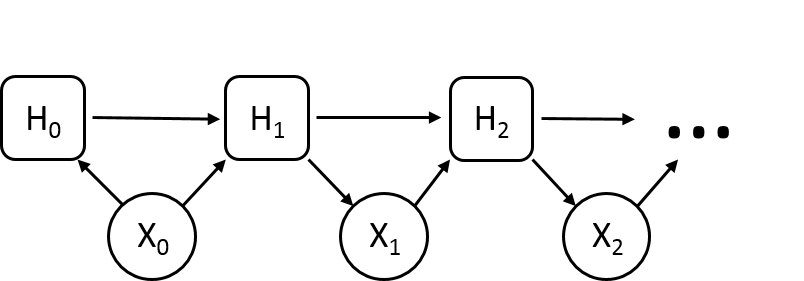
\includegraphics[width=0.3\textwidth]{gsn_computational_graph}
%\caption{GSN computational graph.}
%\end{figure}

The latent state variable \(H\) can be equivalently defined as \(H_{t+1} = f_{\Theta_1}(X_t,Z_t,H_t)\), a learned function \(f\) with an independent noise source \(Z_t\) such that \(X_t\) cannot be reconstructed exactly from \(H_{t+1}\). If \(X_t\) could be recovered from \(H_{t+1}\), the reconstruction distribution would simply converge to the Dirac at \(X\). Denoising auto-encoders are therefore a special case of GSNs, where \(f\) is fixed instead of learned.

GSNs also use the notion of walkbacks to aid training. Walkbacks are the process of generating samples by iteratively sampling from \(P_{\Theta_1}(H|H_t, X_t)\) and \(P_{\Theta_2}(X|H_{t+1})\) for a given input. By using walkbacks, the model is more likely to seek out spurious modes in the data distribution and correct for them \cite{bengio13a}. The resulting Markov chain of a GSN is inspired by Gibbs sampling, but with stochastic units at each layer that can be backpropagated \cite{rezende14}.

\begin{figure}[h!]
  \centering
    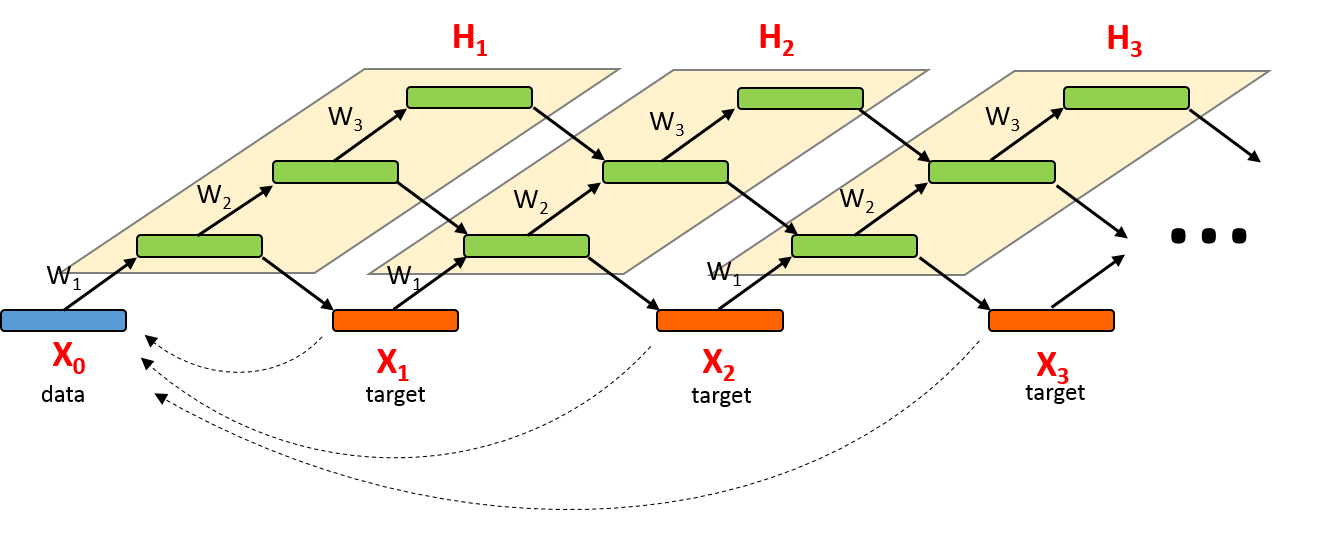
\includegraphics[width=0.5\textwidth]{gsn_markov_chain}
\caption{Unrolled GSN Markov chain.}
\end{figure}

Experimental results with GSNs show that their latent states mix well between the major modes of the data - mixing faster at higher layers in the model \cite{gsn}. Using this property, we tested a simple temporal GSN model to predict sequences of inputs. The temporal GSN uses a linear transformation \(H \rightarrow H\) to predict \(P(H_t|H_{t-1},...,H_{t-n})\) with an input history of size \(n\). Using this predicted \(H_t\), an expected input \(x_t\) was sampled from the model's learned reconstuction distribution \(P_{\Theta_2}(X|H)\).

Qualitatively, this model appears to predict temporal dependencies well within its history window \(n\) (Figure 3). This result provided motivation to use the latent state \(H\) as the emitted parameter in a better-suited temporal model, such as an RNN.

\begin{figure}[h!]
  \centering
    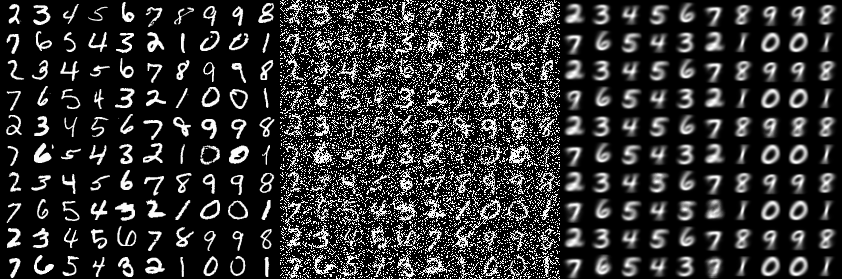
\includegraphics[width=0.5\textwidth]{tgsn}
\caption{Temporal GSN with history \(n=2\) trained on an arbitrary MNIST sequence. Original input sequence is on the left, a noisy version of the input fed into the model is in the middle, and the predicted input based on the history is on the right.}
\end{figure}


\section{Recurrent Neural Networks}
\label{rnn}
Traditional RNNs simulate a discrete-time system that has an input sequence \(\{x_1...x_t\}\) and a hidden state sequence \(\{h_1...h_t\}\) that map to an output sequence \(\{y_1...y_t\}\). The network is defined for timestep \(t\) in the sequence by the hidden and output equations:
\begin{equation}
	h_t = \Phi_h(W^Th_{t-1} + U^Tx_t + b_h)
\end{equation}
\begin{equation}
	y_t = \Phi_y(V^Th_t + b_y)
\end{equation}
where \(\Phi_h\) and \(\Phi_y\) are element-wise nonlinear functions and \(W\), \(U\), \(V\), \(b_h\), and \(b_y\) are the network parameters.



\subsection{Extension to deep RNN}



\section{The RNN-GSN}
\label{rnn-gsn}
This is the main RNN-GSN section.


\section{Experiments}
\label{experiments}
We experimented with the RNN-GSN described by Algorithm \ref{algo} on sequences of MNIST images and standard MIDI datasets.
Each RNN-GSN was first initialized with GSN parameters and trained with noise scheduling, which has been shown to help the network learn appropriate features during stochastic gradient descent \cite{noise_schedule}.

The GSNs used $1500$ hidden units, $3$ hidden layers, and $5$ walkbacks, and the RNNs used $1500$ hidden units and $1$ hidden layer. $Tanh$ activation was used for hidden units, $sigmoid$ activation for visible inputs, and the network was trained using stochastic gradient descent on a binary cross-entropy cost with momentum of $0.5$ on the parameters and annealing of $0.995$ on the learning rate starting at $0.25$. GSN noise was added as salt-and-pepper, starting at $0.7$ with a schedule rate of $0.98$. MNIST input dimensionality is 784 and MIDI input dimensionality is 88.
\subsection{Sequences of MNIST digits}
The MNIST dataset is a series of greyscale handwritten digits. To introduce a temporal structure, we created three increasingly complex sequences of images. Log-likelihoods are estimated by a Parzen density estimator, which is biased. Further validation can be seen qualitatively by the predicted samples produced from the models.

\textbf{Sequence1} is a simple linear sequence of digits \{0,1,2,3,4,5,6,7,8,9,...\} repeating. As seen with the TGSN example in Figure \ref{fig:tgsn}, this sequence can be modeled as a linear transformation in the hidden state space $H$ of the GSN. The RNN-GSN is also able to model this sequence, achieving a mean Parzen log-likelihood estimate of $-295.51 \pm 1.5$. From Figure \ref{fig:s1}, the output sequence looks like an expectation over the digits in the correct mode of the input space.
\begin{figure}[h!]
  \centering
    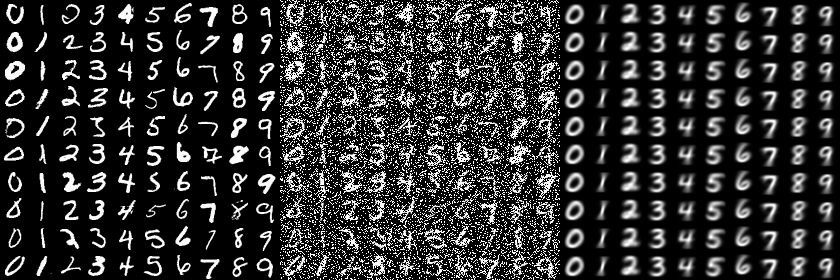
\includegraphics[width=0.5\textwidth]{s1}
\caption{RNN-GSN trained without noise scheduling on Sequence1 after 107 training epochs. Original sequence is on the left, noisy input to the model is in the middle, and output expected sequence is on the right.}\label{fig:s1}
\end{figure}

\textbf{Sequence2} introduces one bit of parity by alternating the sequences \{0,1,2,3,4,5,6,7,8,9,9,8,7,6,5,4,3,2,1,0...\} repeating, where the next value depends on whether the sequence is ascending or descending. The RNN-GSN is able to model this sequence as well, achieving a mean Parzen log-likelihood estimate of $-221.32 \pm 1.4$. The model was trained both with and without noise scheduling, and the outputs are compared in Figures \ref{fig:s2a} and \ref{fig:s2b}.
\begin{figure}[h!]
  \centering
    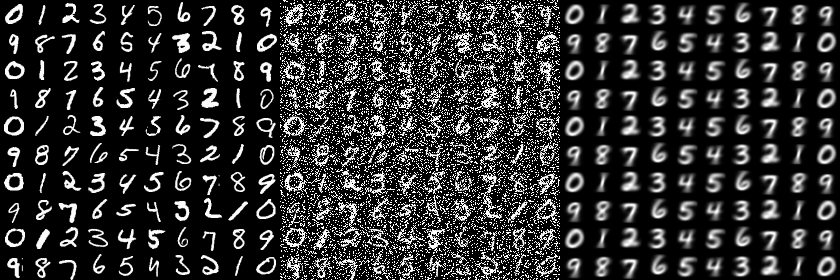
\includegraphics[width=0.5\textwidth]{s2a}
\caption{RNN-GSN trained without noise scheduling on Sequence2 after 132 training epochs. Original sequence is on the left, noisy input to the model is in the middle, and output expected sequence is on the right.}\label{fig:s2a}
\end{figure}
\begin{figure}[h!]
  \centering
    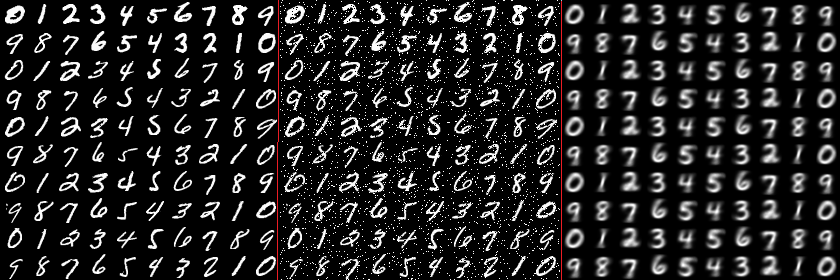
\includegraphics[width=0.5\textwidth]{s2b}
\caption{RNN-GSN trained with noise scheduling on Sequence2 after 115 training epochs. Original sequence is on the left, noisy input to the model is in the middle, and output expected sequence is on the right.}\label{fig:s2b}
\end{figure}


\textbf{Sequence3} creates a longer, more complex sequence by using multiple bits of parity. It is formed by Algorithm \ref{alg:s3}:
\begin{algorithm}
\caption{Sequence3}\label{alg:s3}
\begin{algorithmic}
	\STATE $sequence \Leftarrow [0,1,2]$
	\WHILE{not stop}
		\IF {$sequence[-3]$ is odd}
			\STATE $first\_bit = (sequence[-2] - sequence[-3])\%10$
		\ELSE
			\STATE $first\_bit = (sequence[-2] + sequence[-3])\%10$
		\ENDIF
		\IF {$first\_bit$ is odd}
			\STATE $second\_bit = (sequence[-1] - first\_bit)\%10$
		\ELSE
			\STATE $second\_bit = (sequence[-1] + first\_bit)\%10$
		\ENDIF
		\IF {$second\_bit$ is odd}
			\STATE $next\_num = (sequence[-1] - second\_bit)\%10$
		\ELSE
			\STATE $next\_num = (sequence[-1] + second\_bit)\%10$
		\ENDIF
		\STATE $sequence$ append $next\_num$
	\ENDWHILE
\end{algorithmic}
\end{algorithm}
This sequence has a length of 62 digits, which is longer than most conventional RNNs can learn without special techniques. As shown in Figure \ref{fig:s3}, the RNN-GSN can model the sequence fairly well and achieves a mean Parzen log-likelihood estimate of $-28.46 \pm 1.2$.
\begin{figure}[h!]
  \centering
    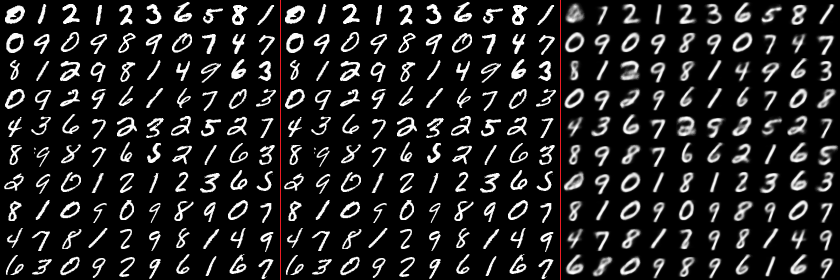
\includegraphics[width=0.5\textwidth]{s3}
\caption{RNN-GSN trained with noise scheduling on Sequence3 after 500 training epochs. Original sequence is on the left, noisy input to the model is in the middle, and output expected sequence is on the right.}\label{fig:s3}
\end{figure}

For reference, the Parzen estimate of a 3-layer, 5-walkback GSN trained on MNIST is $120 \pm 0.8$, and the Parzen estimate of using MNIST train samples is $24 \pm 1.6$.

The RNN-GSN trained on Sequence3 probably has a higher Parzen estimate because the dataset is significantly reduced in size due to the constraint in generating the sequence.

\subsection{Sequences of polyphonic music}
	We applied the RNN-GSN to probabilistic modeling of sequences of polyphonic music as MIDI files. Each dataset was used as described in \cite{rnnrbm}:

\textbf{Piano-midi.de} is a classical piano MIDI archive.\\
\textbf{Nottingham} is a collection of folk tunes.\\
\textbf{MuseData} is a library of orchestral and piano classical music from www.musedata.org.\\
\textbf{JSB chorales} is the corpus of 382 four-part harmonized chorales by J. S. Bach.
	
Log-likelihoods estimated by the Parzen density estimator are biased and cannot be compared to the AIS estimation used by Boulanger-Lewandowski et al. RNN-GSN Parzen estimates are provided in Table \ref{tab:parzen}.
%However, accuracies as computed by Bay et al. are provided for comparison in Table \ref{tab:midi} \cite{bay}.

%\begin {table}[H]
 %\caption {MIDI accuracy \%} \label{tab:midi}
%\begin{tabular}{l | l l l l}
%\hline
%Model & Piano-midi & Nottingham & Muse & JSB\\
%\hline
%RNN-RBM & 28.92 & 75.40 & 34.02 & 33.12\\
%RNN-GSN  & xx.xx  & xx.xx  & xx.xx  & xx.xx\\
%\hline
%\end{tabular}
%\end{table}

\begin {table}[H]
 \caption {MIDI accuracy \%} \label{tab:parzen}
\begin{tabular}{l | l l l l}
\hline
Model & Piano-midi & Nottingham & Muse & JSB\\
\hline
RNN-GSN  & $6.85 \pm 0.23$ & $22.54 \pm 0.14$ & $22.89 \pm 0.08$ & $21.82 \pm 0.16$
\end{tabular}
\end{table}

One important difference to note: the RNN-RBM uses the visible input $x$ when constructing the RBM for each timestep, and the RNN emits the bias parameters $b_h$ and $b_x$. Essentially, the RNN-RBM evaluates $P(X=x_t|H,b_t)$ for each timestep.
The RNN-GSN, on the other hand, only uses the hidden state $H_t$ emitted by the RNN to construct an expected input $\hat{x}_t$ for each timestep, sampling from the GSN's learned distribution $P(X|H)$. This means the predicted input at timestep $t$ is an expected value of the distribution $P(X|H_t)$. For a different accuracy measure, $P(X=x_t|H_t)$ could have been evaluated as well.



\section{Conclusion}
\label{conclusion}
We presented the RNN-GSN, a generative, non-probabilistic model for learning deep sequence representations. We validated its efficacy as a deep recurrent model on complex inputs with sequences of MNIST images and MIDI representations of polyphonic music. The RNN-GSN works as well as other deep recurrent models, such as the RNN-RBM, but is an easier framework to perform inference over and sample from due to its non-probabilistic nature.

Further improvements and areas of study could be using LSTM units in the RNN or Hessian-free optimization, and combining depth at multiple stages of the RNN. We would like to look into using GSNs as both the input-to-hidden and hidden-to-output functions of the RNN, further reducing the complexity for representing the sequence. Finally, multimodal GSNs could provide benefits when the hidden representations of the input data distribution cannot be assumed as unimodal \cite{multi_gsn}.


% Acknowledgments should only appear in the accepted version. 
%\section*{Acknowledgments} 
 %We would like to thank the developers of the Theano framework \cite{theano1, theano2}. We also thank Li Yao, Sherjil Ozair, and Nicolas Boulanger-Lewandowski for their helpful discussions, insight, and code.


% In the unusual situation where you want a paper to appear in the
% references without citing it in the main text, use \nocite
%\nocite{langley00}

\bibliography{references/rnngsn_bibliography}
\bibliographystyle{icml2015}

\end{document}

